\documentclass{article}
\usepackage{tikz}

\title{Averages}
\author{Alex Katsenelenbogen}

\setlength{\voffset}{-0.75in}

\begin{document}
\begin{center}
      \Large\textbf{Inscribed Shapes}\\
      \large\textit{Prepared by Alex Katsenelenbogen}
\end{center}

\vspace{10 mm}



\begin{center}
\begin{tikzpicture}
\draw[line width=0.5mm]  [fill=gray] (1,3) circle (1.4142cm);
\draw [line width=0.5mm] [fill=white]   (0,2) -- (2,2) -- (2,4) -- (0,4) -- (0,2);
\end{tikzpicture}
\end{center}
\begin{enumerate}
\item The circle above has a circumference of $20\pi$ , what is the area of the shaded region?
\item A rectangle is inscribed in a circle where the length is three times its height. If the circle has an area of $225\pi$, then what is the area of the rectangle?
\item A circle is inscribed in a square. If the square has an area of 64$in^2$, what is the circle's area? What is the circle's circumference?
\end{enumerate}




\end{document}
